\subsection{OR問題を学習させた際の誤差収束度合いについて}
\subsubsection{実験結果}
NNでは重みを更新する毎に誤差が減るように学習を行うが、
その学習の様子は初期の重みをどのように設定したか、
学習に用いたパラメータをどのように設定したか、
といった対象問題以外の要素に影響して学習の様子が変化する。
シード値を変えた際の学習収束回数を表\ref{table:level1}に示す。
シード値を10回変更して学習させた際の重みを更新する様子を図
\ref{fig:level1-1}に、
その平均をプロットした平均推移値を図\ref{fig:level1-2}に示す。
なお、平均値を求める際には10種類のシード値における各回数目を加算して10で割ることで平均値を算出した。
具体的にはシェルスクリプトにて、1000 - 10000までのシード値の学習収束回数の各1回目を取り出した後に加算し、10で割る。その結果を"total_ave.dat"に">>"で入力すれば、一回目の平均が算出される。これを100回目まで続けることにより、各シード値における学習収束回数の平均推移値を算出することが出来る。

\begin{table}[htb]
 \begin{center}
  \caption{OR問題の学習に要した回数}
  \label{table:level1}
  \begin{tabular}[htb]{r|l} \hline
   シード値 & 収束した回数 \\ \hline \hline
   1000 &  96\\ \hline
   2000 &  90\\ \hline
   3000 &  111\\ \hline
   4000 &  109\\ \hline
   5000 &  93\\ \hline
   6000 &  99\\ \hline
   7000 &  100\\ \hline
   8000 &  114\\ \hline
   9000 &  113\\ \hline
   10000 & 94 \\ \hline \hline
   10試行の平均値 & 102 \\ \hline
  \end{tabular}
 \end{center}
\end{table}


\begin{figure}[h]
 \begin{center}
  \includegraphics[width=10.0cm]{figs/level1-1.eps}
  \caption{重みを更新する様子}
  \label{fig:level1-1}
 \end{center}
\end{figure}

\begin{figure}[h]
 \begin{center}
  \includegraphics[width=10.0cm]{figs/level1-2.eps}
  \caption{重みを更新する様子(平均値)}
  \label{fig:level1-2}
 \end{center}
\end{figure}


\subsubsection{考察}
学習回数が増加する程誤差は収束していくが、終始右肩下がりというわけではなく、学習序盤に誤差の値が上下しながら収束していきます。学習回数が少ないうちは誤差の変化が大きく、学習回数が多くなっていく程誤差の変化は小さくなっていくと考えられます。


